\begin{frame}[fragile]
        \frametitle{Database example}
Database is collection of tables
\begin{itemize}
    \item Table contains rows and columns
    \item Tables may have relationships
\end{itemize}

Activities Table
\begin{tabular}{| c | c | c | c | c |}
   \hline
   Student     & Activity1 & Cost1 & Activity2 & Cost2 \\ 
   \hline 
   John Smith  & Tennis    & \$36  & Swimming  & \$17  \\
   Jane Bloggs & Squash    & \$40  & Swimming  & \$17  \\
   John Smith  & Tennis    & \$36  &           &       \\
   Mark Antony & Swimming  & \$15  & Golf      & \$47  \\ 
   \hline
\end{tabular}

\end{frame}

\begin{frame}[fragile]
        \frametitle{Database example}
        \center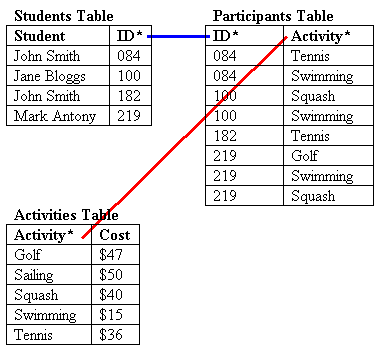
\includegraphics[width=0.7\textwidth]{../../slides/web/media/db_table.png}
\end{frame}
